\section{Design}

\subsection{System Layers}
The user must be able to access the app via a web browser.

It was decided that the TV and programme streams should be delivered to the client via Wowza media server, which would be hosted on a machine running Windows Server 2008. Peter Wood (Inqb8r) has had extensive experience with Wowza, and assisted Dexter in the configuration of the server to output the Channel 4 streams. This helped by relieving us of any lengthy configuring that might have had to take place with any other system. Additionally, Inqb8r were able to provide us with a licensed Wowza server.

LAMP server

\subsection{Personalised TV Channel}

\subsection{Programme Recommendation}
	A your4.tv user is presented with a personal channel populated with a list of programmes as recommended by a programme recommendation system.  This system only recommends programmes, and is separate from the targeted advert retriever (described in Section~\ref{sec:design_adverts}). At an abstract level, each programme is given a vector $\mathbf{p}$, which describes what the programme is like. The programme vector $\mathbf{p}$ lies within the programme space $\mathcal{P}$, and is calculated from a vector of programme information $\mathbf{i}$ using the function $v_p$ ($\mathbf{p} = v_p(\mathbf{i})$). The concrete implementation of this used in your4.tv is that $\mathcal{P}$ is 19-dimensional, where each dimension represents one of the genres:
	\begin{center}
		\emph{\footnotesize{
			\begin{tabular}{c c c c c}
				Action and Adventure & Animation & Children & Comedy & Documentary \\
				Drama & Game Show & Home and Garden & Mini-Series & News \\
				Reality & Science-Fiction & Fantasy & Soap & Special Interest \\
				Sport & Talk Show & Western & Unclassified & 
			\end{tabular} 
		}}
	\end{center}
	which is the full set of allowable genres on The Tvdb\footnote{\footurl{http://thetvdb.com}} plus `Unclassified', which is reserved for programmes which $v_p$ cannot assign an appropriate vector. To map a programme into this space, $v_p$ uses the supplied programme name to query the Tvdb API\footnote{\footurl{http://thetvdb.com/wiki/index.php/Programmers\_API}} for a programme's genres, and returns a binary vector of genre memberships (for each element: 1 if the programme belongs in genre; 0 otherwise). As an example, the programme `Grand Designs' has genres \emph{Documentary}, \emph{Home and Garden} and \emph{Reality}, so would be assigned the vector $\left[0,0,0,0,1,0,0,1,0,0,1,0,0,0,0,0,0,0,0\right]^T$.

	So that a user may be recommended programmes, each user is given a vector, $\mathbf{u}$, also within the space $\mathcal{P}$, which represents the users ideal programme. This user vector is initialised with the function $v_u$, which takes a vector of a users demographic information, $\mathbf{d}$, and returns the user vector, $\mathbf{u}$ ($\mathbf{u} = v_u(\mathbf{d})$). The actual demographics in $\mathbf{d}$ are constrained by the target audience, the training data available and the user data available, and as a result only gender is considered ($\mathbf{d} \in \left\{{ \left[ 0\right] ,\left[ 1\right] }\right\} $). The function $v_u$ is learned using a set of training data containing mappings between users, their demographics and shows they enjoy. While a user uses your4.tv, their actions influence their user vector. Upon giving a programme a rating, $\mathbf{u}$ is moved either towards or away from $\mathbf{p}$ by an amount which depends upon the magnitude of the rating, the initial distance between $\mathbf{u}$ and $\mathbf{p}$, and the learning rate of the recommender which may be tweaked or made inversely proportional to the number of ratings made by the user. While an adaptive learning rate will result in a simulated-annealing type search in the programme space, a constant learning rate will continue adapting recommendations to the users current mood, which should not be assumed to be static. The exact change to $\mathbf{u}$, where $\mathbf{u}_{i}$ is the $i^{th}$ component of vector $\mathbf{u}$, $\mathbf{u}'$ is the new user vector, $0 \leq L \leq 1$ is the learning rate and $-1 \leq r \leq 1$ is the rating given is given by:
	% {\left[1\right], \left[0\right]
	% Can use dcases in mathtools to make the fractions in the conditional more readable (bigger).
	$$
		\mathbf{u}_{i}' =
		\mathbf{u}_{i} + \begin{cases}
			\left|\mathbf{p}_{i}-\mathbf{u}_{i}\right|Lr \times \frac{\mathbf{p}_{i}-\mathbf{u}_{i}}{\left|\mathbf{p}_{i}-\mathbf{u}_{i}\right|},&
				\text{if } r\geq 0\\
			(1-\left|\mathbf{p}_{i}-\mathbf{u}_{i}\right|)Lr \times \frac{\mathbf{p}_{i}-\mathbf{u}_{i}}{\left|\mathbf{p}_{i}-\mathbf{u}_{i}\right|},&
				\text{otherwise}
		\end{cases}
	$$
	Because of division by 0 for the case when the user and programme vectors are, on a particular dimension, identical ($\mathbf{p}_{i}-\mathbf{u}_{i}=0$), a special case was required:
	$$
		\mathbf{u}_{i}' =
		\mathbf{u}_{i} + \begin{cases}
			0,&
				\text{if } r\geq 0\\
			\operatorname{sign}(\operatorname{random}()-0.5)\times Lr,&
				\text{otherwise}
		\end{cases}
	$$

	Genres from Tvdb were chosen as a basis for $\mathcal{P}$ instead of the Project4 or Atlas genres, as this solved the problem of finding training data for the learned function $v_u$. No programme viewing data was available using Project4 or Atlas genres, so the MovieLens 1M dataset\footnote{\url{http://www.grouplens.org/node/73}} was downloaded, and the movies mapped to their corresponding Tvdb genres, giving a large dataset of user demographics, movie ratings, and movie vectors within the programme space $\mathcal{P}$ which serve as suitable training data. To map new programmes into the $\mathcal{P}$, $v_p$ looks up the Tvdb genres for a given programme, using these to construct $\mathbf{p}$.

		\begin{figure}[h!]
			\begin{center}
			\begin{subfigure}[t]{0.32\textwidth}
				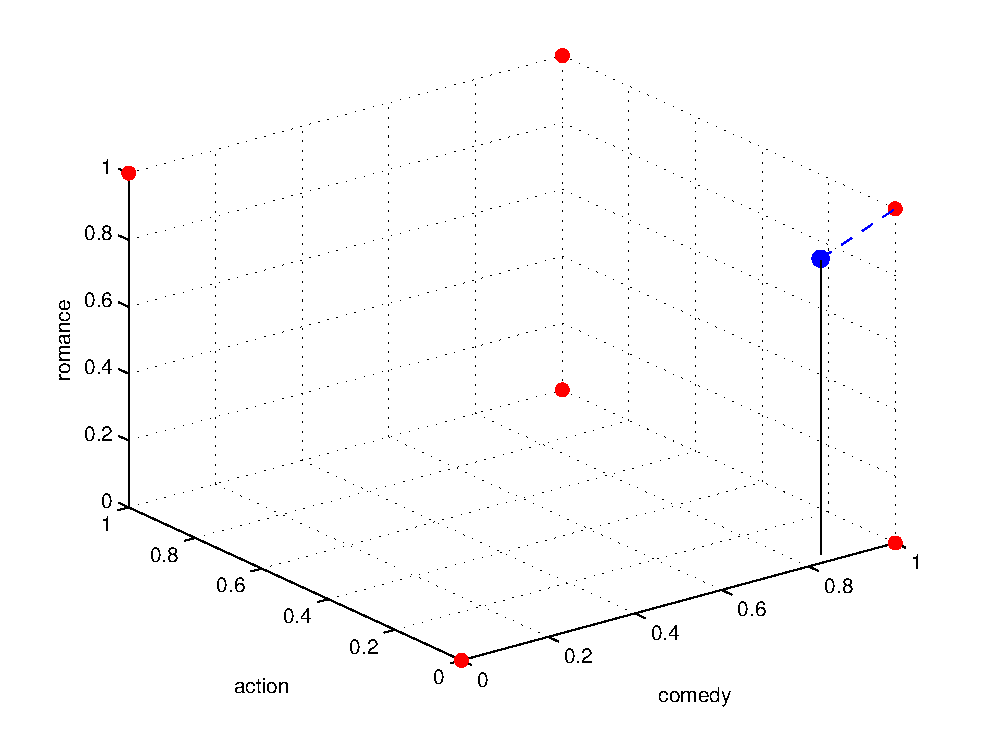
\includegraphics[width=\textwidth]{images/recommender_1.pdf}
				\caption{A user is recommended the programme which minimises $||\mathbf{p} - \mathbf{u}||$.}
			\end{subfigure}
			\begin{subfigure}[t]{0.32\textwidth}
				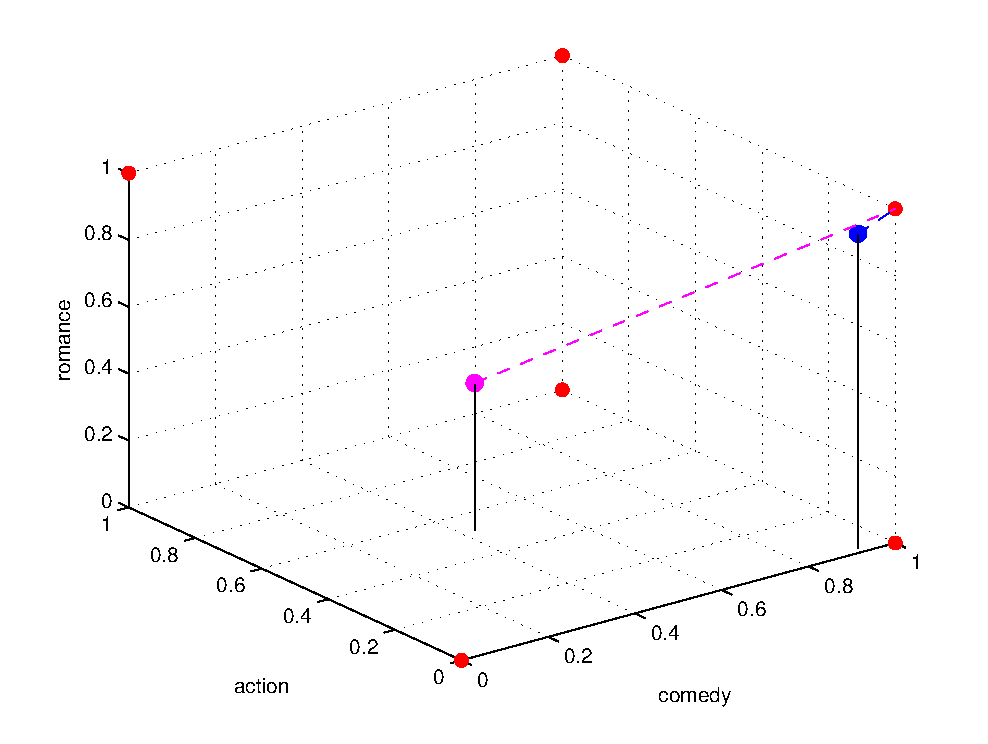
\includegraphics[width=\textwidth]{images/recommender_2.pdf}
				\caption{Giving a rating modifies $\mathbf{p}$. Here, a positive rating results in the blue (righthand) and a negative rating gives the purple (lefthand) pin.}
			\end{subfigure}
			\begin{subfigure}[t]{0.32\textwidth}
				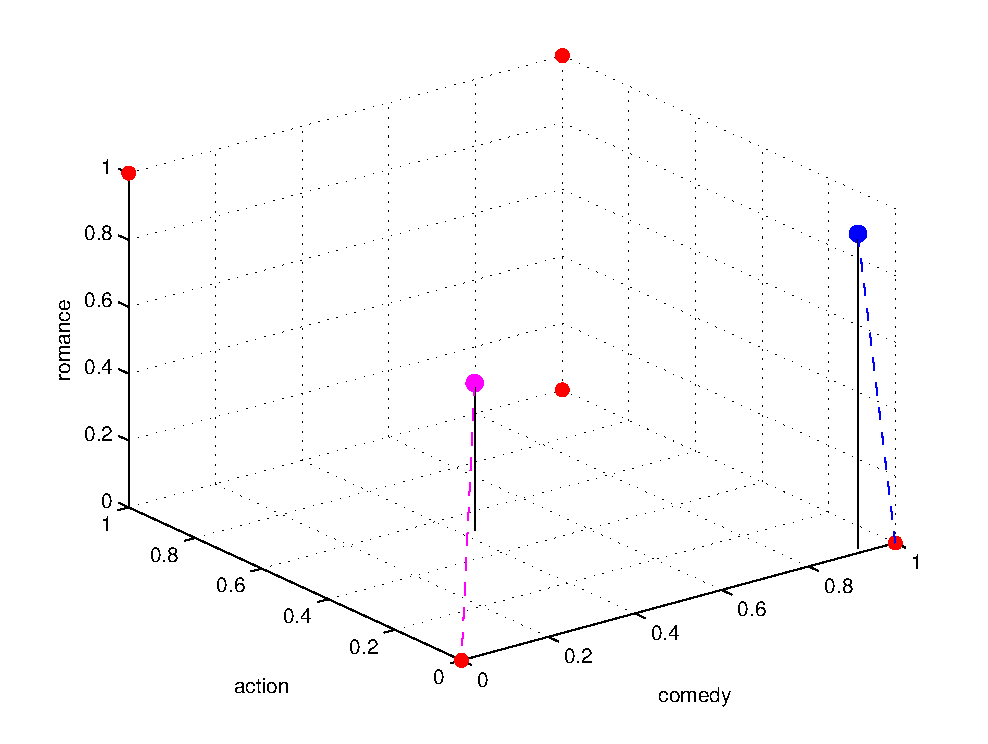
\includegraphics[width=\textwidth]{images/recommender_3.pdf}
				\caption{The programme just watched/skipped is removed from the users programme pool, and the user is recommended a new different programme.}
			\end{subfigure}
			\caption{Visualisation of how the state of an example 3-dimensional version or the recommender described above changes during use. The axes used in this example are romance, action and comedy; a subset of the 18 dimentions in the actual implementation.}
			\label{fig:recommender_example}
		\end{center}
	\end{figure}

	The space $\mathcal{P}$ is, by design, coupled only with the functions $v_u$ and $v_p$. As a result of this, $v_p$ may be modified, changing the structure of $\mathcal{P}$, as long as $v_u$ is re-learnt using the new programme representation. This is desirable, as programme representations better suited to recommendation are possible; i.e., more similar programmes are closer together, more different programmes are further apart, and similar programmes are not given identical representations. Possible ways of accomplishing this are discussed in section~\ref{sec:further_work_recommender}.



\subsection{Granularly Targeted Adverts}
\label{sec:design_adverts}

In [cite] it is discussed that adverts that are relevant to users are more likely to be of interest and in \citet{yahoo-intrusive-advertising} is shown to influence user experience. Furthermore, our prestudy (Section~\ref{sec:prestudy}) revealed that x\% [fixme] of participants would pay more attention to adverts that are relevant to them. The use of granular targeting would allow advertisers to specify very specific target markets, based on demographics, browsing habits and contextual information. As shown in [cite], adverts targeted specifically towards individuals are, in general, more relevant to that individuals personal interests.

The usage of internet-connected devices allows the capturing of information about a user, allowing this granular targeting. In the design of our advertising platform, we take the notion of an advert campaign, as used by [cite] in [some system], and allow an advert to be targeted towards people based on personal information (such as age, gender and occupation), usage data (such as viewing history) and contextual information (such as time of day and what programme they are watching).

[cite] discusses the use of skip functionality in adverts in [system]. Users were able to skip adverts that they did not enjoy, such that they would be presented with a different advert for the remainder of the advert break. x\% of users were satisfied that by skipping adverts, they would be more likely to be presented with adverts that were of interest to them. Furthermore, our prestudy revealed that x\% [fixme] of individuals felt that skip functionality would influence the attention they would pay to adverts. From this, we wish to include skip functionality as part of our design: a user may skip an advert in order to be presented with a different advert, and may do so until the advert break has finished.

In the context of live TV, these targeted adverts would replace adverts that are streamed as part of the channel by the broadcaster. This advert replacement has been implemented successfully previously as part of Project4, as described in Section~\ref{project4}. In addition, these advert breaks could be placed in between non-live streamed programmes.

\subsubsection{Advert campaigns}

Any advert may be targeted towards individuals by assigning that advert to a campaign. An advert may be in as many campaigns as the advertiser needs, and a campaign may include any number of adverts. A campaign is given a set of restrictions, where the adverts belonging to a campaign are shown whenever the restrictions are met. Restrictions may apply to programmes, users and times, where the attributes that can be restricted are:

\begin{center}
	\begin{tabular}{c c r l}
		\toprule
		\textbf{Programmes} & \textbf{Times} & \multicolumn{2}{c}{\textbf{Users}} \\
		\midrule
		genre & time of day & ~~gender & latitude \\ % The two non-breaking spaces are so the table looke a little nicer. ( Nice olde English there )
		individual programme & weekday & age & longitude \\
		liveness & & &  occupation \\
		\bottomrule
	\end{tabular}
\end{center}

Attributes may have multiple restrictions, where the restrictions are discrete points or continuous ranges where appropriate. When a campaign has multiple restrictions on a single attribute, that attribute is considered satisfied if any of its restrictions are satisfied; e.g.: if a campaign has weekday restrictions of Monday and Wednesday, the weekday restriction is considered satisfied on either a Monday or a Wednesday. A campaign only applies when all of its restrictions are satisfied, though a campaign need not have restrictions for all of the above attributes, or indeed any restrictions at all.

Whenever a campaign is satisfied, its adverts are shown with a frequency directly proportional to the value of a campaign metric that we call \textit{nicheness}. We define nicheness, $n$, as:
$$
	n = \frac{(1-n_\text{programme}) + (1-n_\text{time}) + (1-n_\text{user})}{3}
$$

where
\begin{align*}
	n_\text{programme} &= 1 - \frac{\text{satisfying programmes}}{\text{total programmes}} \\
	n_\text{time} &= 1 - \frac{\text{satisfied time during campaign}}{\text{total time during campaign}} \\
	n_\text{user} &= 1 - \frac{\text{satisfying users}}{\text{total users}}
\end{align*}

In other words, for a particular person, programme and time in which multiple campaigns apply, campaigns with a higher nicheness will have their adverts displayed more often. This design decision was made to reward advertisers for creating niche campaigns over broad campaigns. By encouraging a greater number of more highly targeted advertisements in this way, users will be shown a far more relevant advert set.
% DOES our study show this?

\subsubsection{Collection of Statistics}

Users are able to skip an advert, prompting a box asking the reason they chose to skip the advert, where the advert may be blacklisted for the user, depending on their response. Skipping adverts does not reduce the amount of time the user spends watching adverts, instead simply allows the collection of user preference data and replaces the advert for another.


\subsection{Streaming}
The Wowza server will be configured to act as a repeater, re-broadcasting the streams provided by Inqb8r. The Cupertino streaming packetiser will be used to output the streams in the HLS format such that the videos may be viewed on iPads and any other devices supporting this technology. Each programme will be recorded using the EPG data. Since adverts will be replaced by ones recommended to viewers, it must be known when adverts are due to start and finish. This process is achieved by Project4 using a GPI\citep{SCTE104} triggered hardware solution utilising an SCTE 104 Server, a Tanberg Encoder and a PV1000 Ad replacement device as described in \ref{subsubsec:Project4Tech}. Finally the Wowza server will be configured with the standard extension ``vod'' which allows any file of a valid format in a given directory to be streamed.

\subsubsection{Project 4 Advert Replacement: Hardware Solution}\label{subsubsec:Project4Tech}
Ad break information is sent to a Miranda Xplayer Server from Channel 4 via an automation system which forwards this information as XML to a SCTE 104 device. This information is received via HTTP when the SCTE server is running in HTTP Server mode. Ad information is received on this interface 1 minute and 8 seconds before the Ad break is due to start. On receiving this information it checks with a PV1000 substitution device for a matching Ad break, see \citep{PV1000Schedule}. If it finds one it starts listening for a GPI pulse, sent from the automation system which when triggered instructs the Tanberg Encoder which encodes the video stream to insert markers around the ad breaks. This pulse is received 8 seconds before airing. The PV1000 devices then detect these markers and replace the ad break with one they have created\ref{Project4EventFlow}.

\paragraph{PV1000 Schedule}\label{PV1000Schedule}
The PV1000 receives its schedule from the TMS server. The TMS server receives EPG information from the princess server which pulls it from an EPG ftp service. A user uploaded Channel 4 schedule is also provided to the TMS server 2 weeks in advance. The calculated ad breaks are then provided to the PV1000.

\subsubsection{Your4 Advert Replacement: Software Solution}
When the XML data is received defining the ad breaks as described in \ref{subsubsec:Project4Tech} the information (known as a MOS record) is also stored in a MySQL database. This database also includes EPG information We have been given access to this database and thus (excluding network delays) we are able to discover the existence of Ad breaks up to 1 minute and 8 seconds before they are shown. This information will then made available via the your4 REST interface and the clients will use this warning to call the advert recommender to determine which adverts should be shown in place of the existing ones (see Section~\ref{sec:design_adverts}). These adverts will then be streamed as separate files from the Wowza server using the ``vod'' extension.

\subsubsection{Recordings}
The Wowza server will be configured to include the standard extension ``Live Stream Record'' which allows the use of HTTP to record any active streams to a given file. A restriction of this module is that only 1 recording of each stream is permitted. A custom Wowza ServerListener module will be created which will start with the server. This module will continuously poll the your4 REST interface for any shows due to start in the next minute. This information will be retrieved from Atlas in advance by a cron job on the LAMP server as described in \ref{subsec:ScheduledTasks}. When a new show starts any current recording on the channel will be stopped resulting in a streamable file which will be placed in the directory that the ``vod'' extension is configured to use. This file may then be streamed at any time until it is deleted. Once the current recording is stopped a new one will be started to record the new show. By making a new recording end existing recordings we ensure mutual exclusion for each stream, this is required as the ``LiveStreamRecord'' extension only allows a single recorder on each stream. After a configurable period of time the recording will then be removed from the list of recordings but will only be deleted after a further period of time `t' has elapsed where `t' is the length of the video, allowing any existing streamers to finish watching before it is removed. Throughout this process the Wowza module will also use the REST interface to detail the state of any given program where valid states are: ``Not Recorded, Recording, Recorded, Deleted.''

\subsubsection{Restrictions}
Without a GPI trigger millisecond precision is not possible for advert timings but assuming the network delay remains approximately constant second accuracy should be possible in most situations. Unfortunately live shows can result in these times being slightly out so in some cases the information may be incorrect. We have been given access by Inqb8r to the SCTE 104 control scripts which are coded in Python. Using these we should be able to minimise this risk by pinging the Wowza server and the LAMP server when the GPI pulse is received which is precisely 8 seconds before ad ad break is due to start. Additionally this information could be used to start and stop the recordings on the Wowza server resulting in recordings excluding the adverts allowing potential insertion of adverts at the user's discretion, allowing them to choose when to watch the adverts. However due to the lack of an available development device and the difficulty of modifying the scripts to perform our tasks without interfering with the existing Project4 tasks it has been decided that using this information is outside the scope of this project.

\subsection{Interactive Adverts}

In our prestudy, participants revealed they would often use the advert break as an opportunity to perform another task, such as leave the room to make a drink.


